\chapter{Problem Analysis}
\label{problemanalysis}

In the scope of our project, all citations are classified into 2 types: \textbf{General} and \textbf{Specific}. We define citations as such to be inline with our goal. That is, to be able to tell, if Specific, where the cited information is in the cited document. Otherwise, the citation would be deemed General. To rid of ambiguity in our definition of a General/Specific citation, we have the following guidelines:\\
\textbf{General Citations}
\begin{enumerate}
\item Authors may refer to a paper as a whole. If the author cites for a key idea, e.g. Machine Learning, and Machine Learning makes up the entire or majority of the cited paper, it is a general citation.
\item Authors may refer to a paper as a form of mentioning. The authors merely mentions the cited paper out of acknowledgement of its contributions.
\end{enumerate}
\textbf{Specific Citations}
\begin{enumerate}
\item Authors may refer to a term definition in the cited paper.
\item Authors may refer to a key idea/implementation in the cited paper. This key idea/implementation does not make up the entire cited paper.
\item Authors may refer to an algorithm or a theorem in the cited paper. This algorithm/theorem does not make up the entire cited paper.
\item Authors may refer to digits or numerical figures in the cited paper. Usually for making reference to evaluation results in the cited paper. Authors may also complement the cited paper for its promising/excellent performance.
\item Authors may quote a line/segment in the cited paper.
\end{enumerate}

\begin{figure}[h]
\label{fig:terminology}
\framebox[\textwidth]{
	\begin{tabular}{ l p{11cm}}
		\textsc{Term} & \textsc{Description}\\
		\hline
		Citing Paper & The paper that makes the citation \\
		Cited Paper & The paper that is being cited by the citing paper \\
		Cite Link & E.g. \url{E06-1034==>J93-2004}. A citation relation between a citing paper (\url{E06-1034}) and a cited paper (\url{J93-2004}) \\
		Cite String & The citation mark. E.g. Nivre and Scholz (2004), [1], (23) \\
		Citing Sentence & A sentence in the citing paper that contains the in-line citation. E.g. \textit{That algorithm, in turn, is similar to the dependency parsing algorithm of \textbf{Nivre and Scholz (2004)}, but it builds a constituent tree and a dependency tree simultaneously.} \\
		Citing Context & The block of text surrounding the citing sentence, about 2 sentences before and after the citing sentence, for providing contextual information \\
		Cited Fragment & A fragment, from a few lines to paragraphs, in the cited paper
	\end{tabular}
}
\caption{Terminologies used in this paper}
\end{figure}

%In the scope of our project, all citations are classified into 2 types: \textbf{General} and \textbf{Specific}. We define citations as such to be inline with our goal. That is, to be able to tell, if Specific, where the cited information is in the cited document. Otherwise, the citation would be deemed General. To rid of ambiguity in our definition of a General/Specific citation, we have the following guidelines:\\
%\textbf{General Citations}
%\begin{enumerate}
%\item Authors may refer to a paper as a whole. If the author cites for a key idea, e.g. Machine Learning, and Machine Learning makes up the entire or majority of the cited paper, it is a general citation.
%\item Authors may refer to a paper as a form of mentioning. The authors merely mentions the cited paper out of acknowledgement of its contributions.
%\end{enumerate}
%\textbf{Specific Citations}
%\begin{enumerate}
%\item Authors may refer to a term definition in the cited paper.
%\item Authors may refer to a key idea/implementation in the cited paper. This key idea/implementation does not make up the entire cited paper.
%\item Authors may refer to an algorithm or a theorem in the cited paper. This algorithm/theorem does not make up the entire cited paper.
%\item Authors may refer to digits or numerical figures in the cited paper. Usually for making reference to evaluation results in the cited paper. Authors may also complement the cited paper for its promising/excellent performance.
%\item Authors may quote a line/segment in the cited paper.
%\end{enumerate}

In general, for \textbf{Specific} citations, we would be able to specifically extract a fragment in the cited paper that represents the source of the information mentioned in the citation itself i.e. Citation Provenance.

\subsection{Scope Of The Problem}
\paragraph{}
Our problem is now reduced to determining whether a citation is General or Specific. If a citation is General, the reader can be directed, for example, to the Abstract section of the cited paper, but this is not the main focus of our task. If a citation is Specific, the reader can be directed to that specific paragraph or lines respectively. Therefore during computation, the cited document can be broken down into fragments. Hence if given that a citation is Specific, then there must exists a fragment that the citation refers to. For this we need to implement some ranking system that determines the location of this fragment.

\paragraph{}
We abstract away the problem of locating the in-line citations in a paper, and reduce our problem to only determining the type of a citation and its location. To solve the problem of locating the in-line citations, we utilize the open-source ParsCit system developed by \cite{parscit}. Conveniently, ParsCit identifies the citing sentence, together with the citing context.

\subsection{Modelling The Problem As Search}
\paragraph{}
In web search engines, an user enters a search query, and a search engine would use this query to search within its search domain -- millions of web pages -- and then display the best matching web pages as compared to the search query. That would be equivalent to having a search query for an entire corpus of research papers. Our problem can also be modelled as a searching problem, but a reduced version as compared to web search engines.

\paragraph{}
Consider reading a paper, \url{A}. We know the citations made by \url{A}, and these cited papers are listed in the References section of \url{A}. From this our search domain for any query from \url{A} would be the contents of the list of cited papers. We reduce this search domain further when we are investigating a particular citation in \url{A}, say now paper \url{A} cites the paper \url{B}. Now, for this citation, the scope of search would be the sub-domain -- contents of paper \url{B}. So instead of searching for the best matching document in the corpus, we are now searching within \url{B}. Our problem analysis tells that we have to break down \url{B} into fragments, and the search query would be for these fragments (Refer to Figure \ref{fig:model} for a simple illustration). With the help of ParsCit \cite{parscit}, the citing context can be extracted. The search query would be citing context which consists of the citing sentence.

\begin{figure}[h]
  \centering
  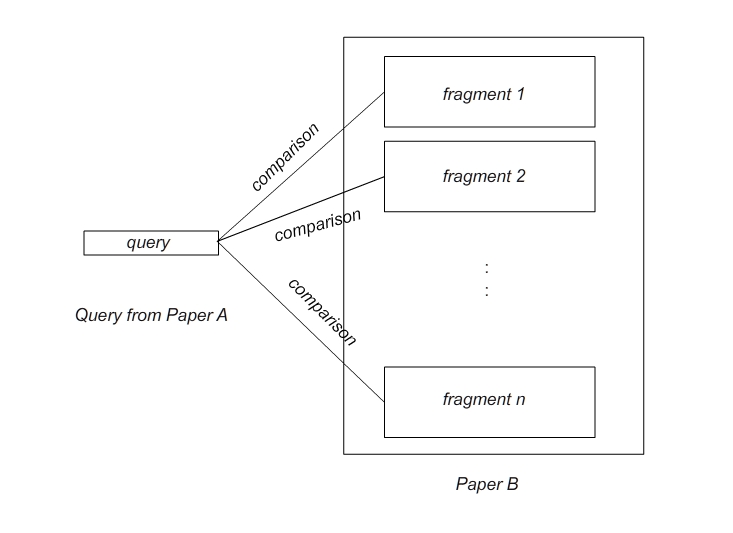
\includegraphics[scale=0.50]{./model}
  \caption{Modeling Our Problem}
  \label{fig:model}
\end{figure}

\paragraph{}
Our problem is now a \textit{binary classification problem}, where we attempt to determine whether a fragment is either General or Specific.

\section{Training Corpus}
\paragraph{}
At this initial stage, we picked the ACL Anthology Reference Corpus\footnote{http://acl-arc.comp.nus.edu.sg/} (ACL-ARC). The ACL-ARC consists of publications of the Computational Linguistics field. Note that in general, we wish to perform this citation provenance task on all publications from all fields of research. This corpus is chosen as a start, because it provides the \textit{interlink data} that conveniently informs us of the cite links between the papers in the corpus. For instance, in the interlink data, a link like \url{X98-103 ==> X96-1049} says that the paper \url{X98-103} cites \url{X96-1049}.

\subsection{Collecting Annotations}
\paragraph{}
Now that we have modelled our problem, we are able to specify the required data format for our task. For each cite link, there can be multiple in-line citations i.e. multiple citing contexts. For each citing context, we are comparing with each fragment in the cited paper. In other words, if a cite link has $n$ citing contexts and the cited paper can be divided into $m$ fragments, immediately we have $(n \times m)$ data instances.

\paragraph{}
Our first attempt at collecting annotations was to require an annotator to specify the line numbers of the cited information that the citing context was referring to. The annotator would be provided the citing and cited paper in plain text format, and he/she will need to annotate on a separate file, specifying the line number range, e.g. line range \url{L12-55} of the cited paper. For this annotation task, we designed an annotation framework\footnote{http://citprov.heroku.com} where an annotator is presented with an user-friendly interface to select the lines in the cited paper that he/she deem Specific. We posted this task onto the Amazon Mechanical Turk (MTurk\footnote{https://www.mturk.com}) for a few MTurk workers to participate in our annotation task. After a trial round of collection, we reviewed this annotation scheme together with feedbacks from our small group of participants.

\paragraph{}
First, this annotation task is a non-trivial one. Participants must be able to understand the contents of the papers, thus, must be researchers or have some experience in reading scientific papers. While it is possible to target a selected category of MTurk workers for our tasks, the complexity of this annotation task requires participants with research experiences, which could be limited in numbers. Furthermore, most of the annotations collected from MTurk do not agree among the annotators and ourselves. To collect annotations that disagree among annotators most of the time, is not helpful for the problem we are trying to tackle. Thus we abandon collecting annotations via MTurk, and performed annotations manually on our own.

\paragraph{}
Second, this annotation scheme is too tricky, and would also cause us much problem when it comes to evaluation. Consider our implemented system that outputs a prediction for citation provenance in the form of a line number range. It is difficult to judge the correctness of this prediction, say \url{L50-78}, when compared against the annotated \url{L12-55} and that the prediction \textit{overlaps} the annotation by 5 lines. This variable amount of overlap is not definitive at all, and is difficult for us to decide at what extent of overlap only do we consider the prediction correct. Thus we switched to the alternative.

\paragraph{}
Our second attempt is more straightforward. Recall that we use ParsCit for extracting the citing context. ParsCit also divides a paper into logically adequate fragments according to sections, sub-sections, figures and tables etc. So instead of annotating by line number ranges, we annotate each of the fragments of the cited papers. We annotate them with 3 classes: General ($g$), Specific-Yes ($y$) and Specific-No ($n$). To be precise, we annotate $g$ (for all its fragments) if a cite link is deemed General, and $y$ \underline{only} for the fragment(s) that is deemed Specific. For the other fragments that are not Specific, we annotate $n$. Table \ref{tab:annotation} summarises the statistics for annotation. Note that we only display percentage values for Specific instances.

\begin{table}[h]
	\center
	\begin{tabular}{ l | l}
		\textsc{Item} & \textsc{Statistics}\\
		\hline
		No. of Cite Links & 275 (7.6\% Specific) \\
		No. of Fragments & 30943 (0.09\% Specific-Yes, 12.9\% Specific-No)
	\end{tabular}
	\caption{Annotation Statistics}
	\label{tab:annotation}
\end{table}

\paragraph{}
As one can see, Specific citations are very rare. From a machine learning point of view, immediately one can observe that the training data is skewed towards General citations. After prolonged periods of searching for valid Specific citations in our training corpus, we argue that even if we attempt to gather more positive instances, the ratio between General and Specific should remain about the same. This challenging situation we have with our annotations also contributes to our approach to the problem, as we explain in the following section.

\section{A Two-Tier Approach}
\label{twotierapproach}
\paragraph{}
We propose a two-tier approach to our problem. In the first tier, it plays the role of a \textit{filter}, and attempts to filter out the General citations, leaving behind the Specific citations to be passed to the second tier. Figure \ref{fig:twotier} illustrates the flow of our approach.
\begin{figure}[h]
  \centering
  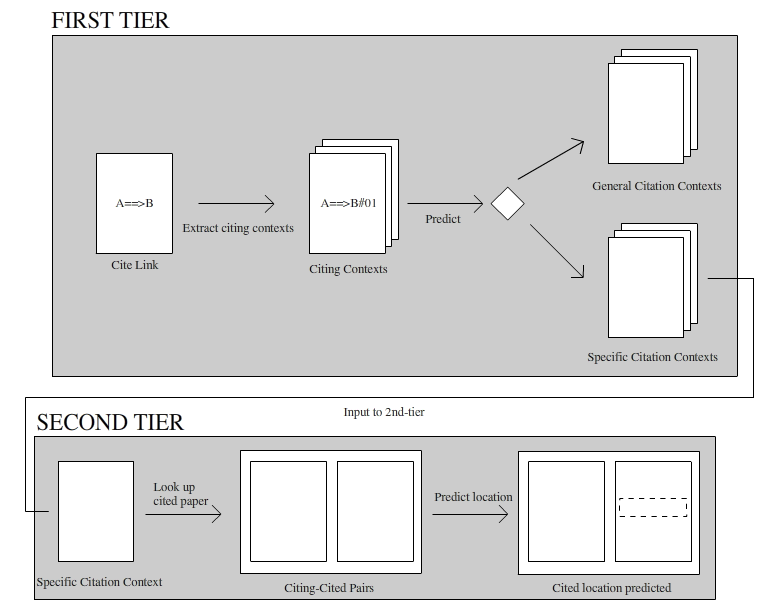
\includegraphics[scale=0.60]{./twotier}
  \caption{A Two-Tier Approach}
  \label{fig:twotier}
\end{figure}

\subsection{First Tier}
\paragraph{}
The First Tier is our attempt to filter out the General citations. In this tier, we are performing a 2-class \textit{citation classification} task, which already is a challenging task in the research area of citation analysis. We are not interested in determining whether the citation is one of the 12 class as defined by \cite{teufel2009annotation}, but only whether it is General or Specific. For each cite link we extract its citing contexts. Then for these contexts we extract feature vectors in order to pass it into our prediction model. We adopt similar features that were presented in previous works on citation classification.

\subsubsection{First Tier Features}
\begin{enumerate}
\item Physical Features \\
We adopted the physical features as presented in \cite{dongensemble}. They are:
\begin{enumerate}
\item \textit{Location}: in which section the citing sentence is from.
\item \textit{Popularity}: no. of citation marks in the citing sentence.
\item \textit{Density}: no. of unique citation marks in the citing sentence and its neighbour sentences.
\item \textit{AvgDens}: the average of Density among the citing and neighbour sentences.
\end{enumerate}

\item Number Density \\
A numerical feature that measures the density of numerical figures in the citing context. The intuition is that Specific citations tend refer to evaluation results in the cited paper. E.g. ``...Nivre and Scholz (2004) obtained a precision of 79.1\%...".

\item Publishing Year Difference \\
A numerical feature that represents difference in the publishing year between the citing and cited paper. The intuition is that higher difference suggests cited paper is older and presented a fundamental idea, and thus cited for General purposes.

\item Citing Context's Average \url{tf-idf} Weight \\
A numerical feature that indicates the amount of \textit{valuable} (as determined by \url{tf-idf} \cite{irtextbook}) words in the citing context. Higher values suggest important words and thus specific keywords.

\item Cue Words \\
Another numerical feature adopted from \cite{dongensemble}, that computes the amount of cue words (pre-defined manually by us) that appear in the citing sentence and its neighbour sentences. We defined 2 classes of cue words: Cue-General and Cue-Specific (refer to Appendix \ref{cuewords} for list of cue words). These cue words are selected based on the examples we observed in our training corpus.
\end{enumerate}
From our training corpus we extracted these features to build our First Tier Model for prediction.

\subsection{Second Tier}
\paragraph{}
In our Second Tier, it is another abstraction of our problem. It is independent from the First tier. We assume all the inputs into the second tier are Specific citations, and then we attempt to predict which of the fragments in the cited paper is the cited fragment.

\subsubsection{Second Tier Features}
\begin{enumerate}
\item Surface Matching \\
A numerical feature that measures the amount of word overlap between the citing sentence and a fragment in the cited paper.

\item Number Near-Miss \\
A numerical feature that measures the amount of numerical figures overlap between the citing sentence and a fragment in the cited paper. This feature will preprocess each fragment, rounding numerical figures or converting to percentage values, when it tries to match the numerical figures in the citing sentence. The intuition for this feature is from our observations that most Specific citations refer to evaluation results in the cited paper.

\item Bigrams Matching \\
A numerical feature that measures the amount of bigrams overlap between the citing sentence and a fragment in the cited paper. This feature is to preserve word order when comparing the citing sentence and the fragment. This feature is also targeted at Specific citations that refer to the cited paper for term definitions and quoting.

\item Cosine Similarity \\
A common numerical feature used in information retrieval tasks to measure similarity between the query and a candidate document. In our case, citing sentence and the fragment.
\end{enumerate}
Similarly we extracted these features from our training data to build our Second Tier Model for prediction.